\section[Zähldaten]{Testverfahren für Zähldaten}

\begin{frame}
  {Übersicht}
  \begin{itemize}[<+->]
%    \item Einführung in Verfahren mit \alert{Test-Werten}
    \item Unterschiede in Zähldaten 
    \item Signifikanz und Effektstärke
    \item Unterschiede bei Ja\slash Nein-Experimenten
  \end{itemize}
\end{frame}

\begin{frame}
  {Literatur}
  \begin{itemize}
    \item \cite{GravetterWallnau2007}
    \item \cite{BortzLienert2008}
  \end{itemize}
\end{frame}

%\subsection{Nichtparametrisch}
%
%\begin{frame}
%  {Nicht-parametrische Tests}
%  \begin{itemize}[<+->]
%    \item Erforderliche \alert{Verteilungsparameter} für Variablen in vielen Tests:
%      \begin{itemize}[<+->]
%	\item normalverteilt
%	\item Varianzhomogenität der Gruppen
%      \end{itemize}
%    \item Vortests auf solche \alert{Verteilungsparameter}:
%      \begin{itemize}[<+->]
%	\item Normalität: \zB Shapiro-Wilk-Test
%	\item Varianzhomogenität: \zB Bartlett-Test
%      \end{itemize}
%    \item Nichtparametrische Tests: keine solchen Voraussetzungen
%    \item Korpusstudien: oft \alert{Zähldaten}, weniger oft Intervalldaten.
%  \end{itemize}
%\end{frame}

\subsection{Vierfelder-Unterschiedstest}

\begin{frame}{Kreuztabelle}
  Beobachtungen von zwei \alert{kategorialen Variablen}.\\
  Auxiliarwahl beim Perfekt: haben, sein\\
  Herkunft des Belegs: nord, sued\\

\begin{figure}[h]
  \centering
  \begin{tabular}{ccc}
    \textbf{Fall} & \textbf{Aux} & \textbf{Region} \\
          1       & haben        & nord   \\
          2       & haben        & nord   \\
          3       & sein         & nord  \\
          4       & sein         & sued  \\
          5       & sein         & sued   \\
          6       & haben        & nord   \\
          7       & haben        & sued   \\
          8       & haben        & sued  \\             
  \end{tabular}
  \onslide<2->{
    \begin{tabular}{|c|c|c|}
      \hline
      & \multicolumn{2}{c|}{\textbf{Aux}}\\
      \hline
      \textbf{Region}      &  haben & sein\\
      \hline
	nord   &   3     &   1\\
      \hline
	sued   &    2    &   2\\
      \hline
    \end{tabular}}
\end{figure}
\end{frame}


\begin{frame}{Kreuztabelle mit Randsummen}

  Spaltensumme für Spalte $i$: \alert{$\sum\limits_{k}x_{ik}$}\\
  Zeilensumme für Zeile $j$: \alert{$\sum\limits_{k}x_{kj}$}\\

\begin{figure}[h]
  \centering
  \begin{tabular}{|c|c|c||c|}
    \hline
    &  haben & sein & Zeilensummen\\
    \hline
    nord   &   3     &  1   & \onslide<2->{\gruen{4}} \\
    \hline
    sued   &    2   &   2   &  \onslide<3->{\gruen{4}}\\
    \hline
    \hline
    Spaltensummen &   \onslide<4->{\rot{5}}   &  \onslide<5->{\rot{3}} & \onslide<6->{\textbf{8}}\\
    \hline
  \end{tabular}
\end{figure}
\end{frame}


\begin{frame}{Beobachtete vs.\ erwartete Häufigkeiten}

  n=100\\
  50 mal \textit{haben}, 50 mal \textit{sein} (= \alert{Spaltensummen})\\ 
  50 mal Norden, 50 mal Süden (= \alert{Zeilensummen})\\

  \begin{itemize}
    \item<2-> erwartete Häufigkeiten unter Annahme der \Null\\
    = kein Zusammenhang zwischen Hilfsverb und Region?
  \end{itemize}

  \begin{figure}[h]
  \centering
  \begin{tabular}{|c|c|c||c|}
    \hline
	  &  haben & sein & Zeilensummen\\
    \hline
      nord   &  \onslide<3>{25}      &  \onslide<3>{25}    & \onslide<1->{\gruen{50}} \\
    \hline
      sued   &   \onslide<3>{25}      &  \onslide<3>{25}    &  \onslide<1->{\gruen{50}}\\
    \hline
    \hline
     Spaltensummen &  \onslide<1->{\rot{50}}   & \onslide<1->{\rot{50}}  & \textbf{100}\\
    \hline
  \end{tabular}
  \end{figure}
\end{frame}


\begin{frame}{Beobachtete vs.\ erwartete Häufigkeiten}
    n=100\\
    50 mal \textit{haben}, 50 mal \textit{sein} (= \alert{Spaltensummen})\\
    30 mal Norden, 70 mal Süden (= \alert{Zeilensummen})\\

  \begin{itemize}
    \item<1-> erwartete Häufigkeiten unter Annahme der \Null?
  \end{itemize}

  \begin{figure}[h]
    \centering
    \begin{tabular}{|c|c|c||c|}
  \hline
	&  haben & sein & Zeilensummen\\
  \hline
    nord   &  \onslide<6->{15}      &  \onslide<7->{15}    & \onslide<2->{\gruen{30}} \\
  \hline
    sued   &   \onslide<8->{35}      &  \onslide<9->{35}    &  \onslide<3->{\gruen{70}}\\
  \hline
  \hline
   Spaltensummen &  \onslide<4->{\rot{50}}   & \onslide<5->{\rot{50}}  & \textbf{100}\\
  \hline
    \end{tabular}
  \end{figure}
\end{frame}


\begin{frame}
  {Beobachtete vs.\ erwartete Häufigkeiten}
  \vspace{-1cm}
  n=100\\
  30 mal Norden, 70 mal Süden\\
  40 mal \textit{haben}, 60 mal \textit{sein}\\

  \begin{figure}[h]
  \centering
    \begin{tabular}{|c|c|c||c|}
      \hline
      &  haben & sein & Zeilensummen\\
      \hline
      nord   &  \onslide<2->{12}      &  \onslide<3->{18}    & \onslide<1->{\gruen{30}} \\
      \hline
      sued   &   \onslide<4->{28}      &  \onslide<5->{42}    &  \onslide<1->{\gruen{70}}\\
      \hline
      \hline
      Spaltensummen &  \onslide<1->{\rot{40}}   & \onslide<1->{\rot{60}}  & \textbf{100}\\
      \hline
    \end{tabular}
  \end{figure}

  \begin{center}
    Allgemein: erwartete Häufigkeit für Zellen: $\frac{Spaltensumme \cdot Zeilensumme}{n}$\\[2ex]
    bzw.: \alert{$EH(x_{ij})=\frac{\sum\limits_{k}x_{ik}\cdot\sum\limits_{k}x_{kj}}{n}$}
  \end{center}
\end{frame}


\begin{frame}
  {Beobachtete vs.\ erwartete Häufigkeiten}
beobachtete Häufigkeiten für eine DeReKo-Stichprobe (\textit{geschwebt}):

  \begin{figure}[h]
    \centering
    \begin{tabular}{|c|c|c||c|}
  \hline
	&  haben & sein & Zeilensummen\\
  \hline
    nord   &  27      & 33    & \onslide<1->{\gruen{60}} \\
  \hline
    sued   &   3      & 34    &  \onslide<1->{\gruen{37}}\\
  \hline
  \hline
   Spaltensummen &   \onslide<1->{\rot{30}}   &  \onslide<1->{\rot{67}} & \textbf{97}\\
  \hline
    \end{tabular}
  \end{figure}
  \pause

  erwartete Häufigkeiten:
  \begin{figure}[h]
    \centering
    \begin{tabular}{|c|c|c||c|}
  \hline
	&  haben & sein & Zeilensummen\\
  \hline
    nord   & \visible<3->{18.56}  & \visible<3->{41.44} & \onslide<1->{\gruen{60}} \\
  \hline
    sued   & \visible<3->{11.44}  & \visible<3->{25.56} &  \onslide<1->{\gruen{37}}\\
  \hline
  \hline
   Spaltensummen &   \onslide<1->{\rot{30}}   &  \onslide<1->{\rot{67}} & \textbf{97}\\
  \hline
    \end{tabular}
  \end{figure}
\end{frame}


\begin{frame}{Problem}

  \begin{itemize}[<+->]
  \item Beobachtete und erwartete Häufigkeit weichen ab.
  \item \Null: kein Zusammenhang zwischen Region und Aux.
  \item Ab wann ist der Unterschied "`signifikant"'?
    \vspace{\baselineskip}
  \item Ein gemessener Unterschied ist \alert{siginifikant}, wenn er angesichts der Stichprobengröße groß genug ist, dass wir das im Experiment gefundene Ergenbis nur sehr selten (typischwerweise in unter 5\% der Fälle) erwarten würden, wenn er gar nicht bestünde. 
    \vspace{\baselineskip}
  \item Diese 5\% (als \alert{Anteil} 0.05) sind das \alert{Signifikanzniveau}.
  \item In Fishers Philosophie abgekürzt \Sig, nicht wie oft zu lesen "`$\alpha$-Niveau"'.
\end{itemize}
  
\end{frame}


\begin{frame}{$\chi^2$-Unterschiedstest}
  \begin{figure}[h]
    \centering
    \begin{tabular}{|c|c|c|}
  \multicolumn{3}{c}{beobachtet:}\\
  \hline
	&  haben & sein\\
  \hline
    nord   &  27      & 33 \\
  \hline
    sued   &   3      & 34 \\
  \hline
    \end{tabular}~~~
    \begin{tabular}{|c|c|c|}
  \multicolumn{3}{c}{erwartet:}\\
  \hline
	&  haben & sein\\
  \hline
    nord   &  18.56      & 41.44 \\
  \hline
    sued   &  11.44     & 25.56 \\
  \hline
    \end{tabular}
  \end{figure}
\pause
  \begin{center}
    $\chi^2 = \sum \frac{(beobachtet - erwartet)^2}{erwartet}$\\[3ex]
    \pause
    bzw.: \alert{$\chi^2=\sum\limits_{ij}\frac{(x_{ij}-EH(x_{ij}))^2}{EH(x_{ij})}$}
  \end{center}
\end{frame}


\begin{frame}{Berechnung des $\chi^2$-Werts}
  $\chi^2 = \sum \frac{(beobachtet - erwartet)^2}{erwartet}$\\
  \vspace{1cm}

  \begin{center}
    \begin{tabular}{|c|c|c|}
      \multicolumn{3}{c}{beobachtet:}\\
      \hline
      &  haben & sein\\
      \hline
      nord   &  {\gruen{27}}      & {\gruen{33}} \\
      \hline
      sued   &   {\gruen{3}}      & {\gruen{34}} \\
      \hline
      \end{tabular}
      \ \ \ 
      \begin{tabular}{|c|c|c|}
      \multicolumn{3}{c}{erwartet:}\\
      \hline
	    &  haben & sein\\
      \hline
	nord   &  {\gruen{18.56}}      & {\gruen{41.44}} \\
      \hline
	sued   &  {\gruen{11.44}}      & {\gruen{25.56}} \\
      \hline
    \end{tabular}
  \end{center}

  \begin{tabular}{lc@{~}c@{~}c@{~}c@{~}c}
    \visible<2->{$\chi^2$ =} & \visible<2->{\(\frac{(27-18.56)^2}{18.56}\)} & \visible<3->{+~\( \frac{(33-41.44)^2}{41.44}\)} &\visible<4->{+~\( \frac{(3-11.44)^2}{11.44}\)} & \visible<5->{+~\( \frac{(34-25.56)^2}{25.56}\)}&\\
    \visible<6->{$\chi^2$ =} & \visible<6->{3.84} &  \visible<6->{+ ~~~1.72} & \visible<6->{+ ~~~6.23} & \visible<6->{+ ~~~2.79} &  \visible<6->{= ~~\onslide<1->{\alert{14.58}}}
  \end{tabular}
\end{frame}



\begin{frame}
  {Die $\chi^2$-Verteilung}
  Die $\chi^2$-Verteilung für Stichproben\\
  aus Grundgesamtheiten ohne Zusammenhang:
  \begin{center}
    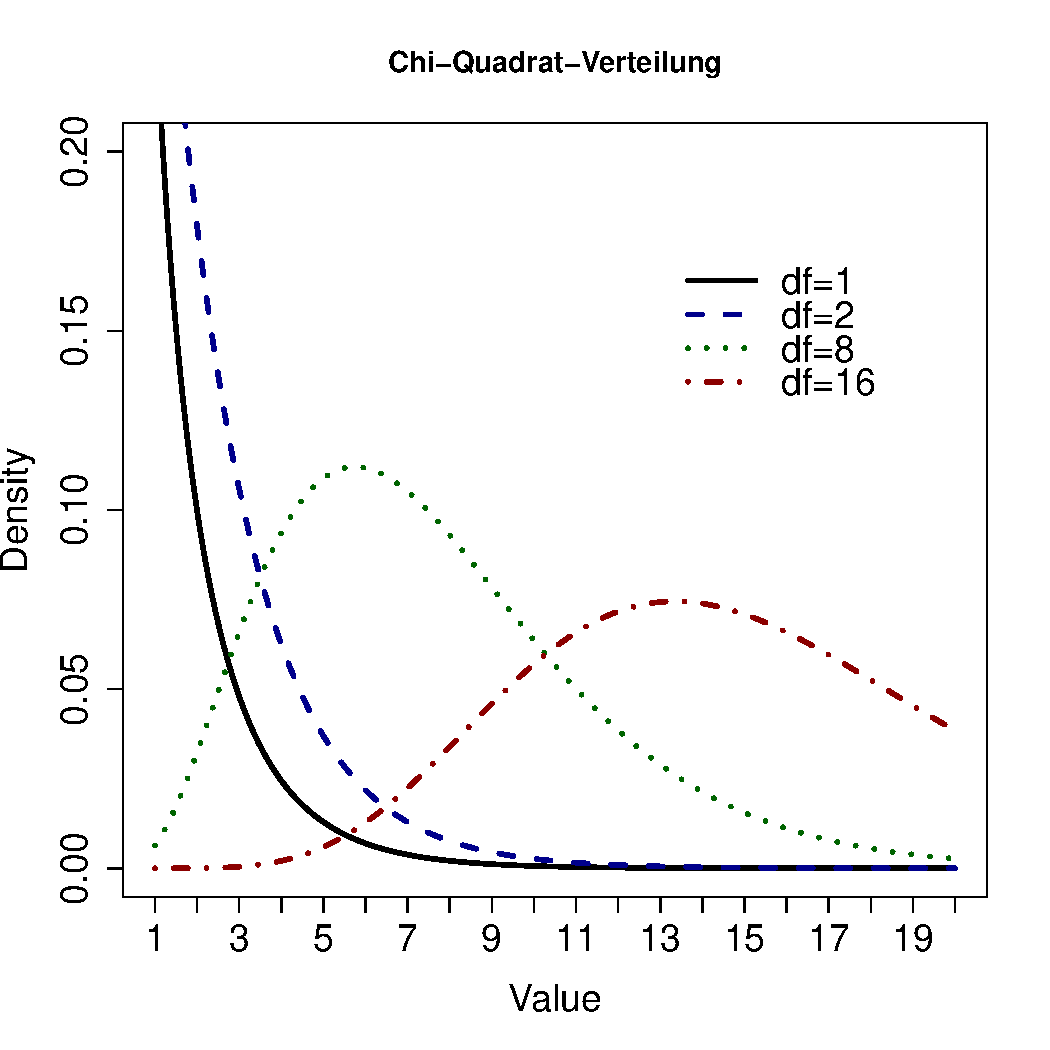
\includegraphics[width=5cm]{graphics/chisq}
  \end{center}
\end{frame}

\begin{frame}
  {Freiheitsgrad?}
  Was sind \alert{"`Freiheitsgrade"'} oder \textit{degrees of freedom (df)}?

  \begin{itemize}[<+->]
    \item Das kommt später noch ausführlicher.
    \item Für n-Felder-Tests: \alert{(Zeilenzahl$-1$)$\cdot$(Spaltenzahl$-1$)}
    \item Bei Vierfelder-Test also: $df=1$
  \end{itemize}
\end{frame}

\begin{frame}{Die $\chi^2$-Verteilung II}
  \begin{itemize}[<+->]
    \item Wahrscheinlichkeit eines bestimmten $\chi^2$-Werts unter Annahme der \Null?\\
      \alert{VOR dem Experiment! Nach dem Experiment ist die Wahrscheinlichkeit\\
      des gemessenen p-Werts immer 1.}
      \vspace{\baselineskip}
    \item In Fishers Philosophie Entscheidung nach \alert{Signifikanzniveau} (\Sig):\\
      \alert{Der $\chi^2$-Wert muss in den extremen \Sig-Anteilen liegen,\\
      um die \Null\ zu \Sig\ zurückzuweisen.}
  \end{itemize}
  \pause
  \begin{center}
    In \texttt{R} ähnlich wie bei Normalverteilung:\\
    \texttt{> qchisq(0.95, df=1) $\Rightarrow$ \texttt{3.84}}
  \end{center}
  \pause
  \begin{itemize}
    \item Also ist für $\chi^2=14.58$ auf jeden Fall $p<0.05$ (weil $14.58>3.84$).
  \end{itemize}
\end{frame}


\begin{frame}
  {Mehr oder weniger signifikant?}
  \begin{itemize}[<+->]
    \item Oft liest man etwas von "`$\alpha$-Niveaus"' wie:
      \begin{itemize}[<+->]
	\item 5\% ("`signifikant"')
	\item 1\%
	\item 0.1\% ("`hochsignifikant"')
      \end{itemize}
    \item Diese Niveaus entsprechen einem falsch interpretierten \Sig.
    \item Die Idee von "`mehr oder weniger signifikant"' ist \alert{kompletter Schwachsinn}.
    \item Entweder ist das gesetzte Niveau akzeptabel,\\
      und dann bringt ein kleineres $p$ aber auch nicht mehr.
    \item Oder es müsste eigtl.\ ein strengeres \Sig-Niveau gewählt werden,\\
      und dann ist $p<0.05$ schlicht nicht ausreichend (s.\ Fishers \alert{Sensitivität}).
    \item Die Entscheidung für ein bestimmtes \Sig-Niveau muss\\
      auf Basis konzeptueller\slash inhaltlicher Gründe gefällt werden.
    \item \alert{EIN signifikantes Testergebnis alleine sagt nicht viel aus!!!}
  \end{itemize}
\end{frame}




\begin{frame}{Voraussetzungen für $\chi^2$-Tests}
  \begin{enumerate}[<+->]
    \item Die Beoabachtungen sind voneinander unabhängig.
    \item In jeder Zelle ist die erwartete Häufigkeit mindestens 5.
    \item Keine Beschränkung auf vier Felder!
  \end{enumerate}
\end{frame}

\begin{frame}
  {In \texttt{R}}
  Mit einer Matrix \texttt{my.matrix}:\\
  \texttt{> chisq.test(my.matrix)}\\
  \vspace{0.5cm}
  
  Eingabe einer einfachen Vierfeldermatrix:\\
  \texttt{> my.matrix <- matrix(c(27,33,3,34), 2, 2, byrow=TRUE)}\\
  \vspace{0.5cm}
  
  Ausgeben der erwarteten Häufigkeiten:\\
  \texttt{> chisq.test(my.matrix)\$expected}\\

  \end{frame}

  \subsection[Fisher-Exakt]{Fisher-Exakt-Test}

\begin{frame}
  {Wann und wie Fisher-Exakt?}
  \alert{Der Fisher-Exakt-Test ist eine Alternative zum $\chi^2$-Test.}\\[3ex]

  \begin{itemize}[<+->]
    \item exakter Test: direkte Berechnung der Wahrscheinlichkeit
    \item \alert{keine} allgemein bessere Alternative zu $\chi^2$
    \item robuster bei sehr kleinen Stichproben
    \item \alert{aber nur für feststehende Randsummen geeignet!}
    \item ohne feste Randsummen: \alert{Barnards Test}
  \end{itemize}
  \vspace{0.5cm}
  
  \visible<4->{
    Fisher-Exakt in \texttt{R}:\\
    \vspace{0.3cm}
    \texttt{> fisher.test(my.matrix)}\\
    \texttt{> fisher.test(my.vector.1, my.vector.2)}
  }
\end{frame}

%\subsection[$\chi^2$ (Anpassung)]{$\chi^2$-Anpassungstest}
%
%\begin{frame}
%  {Situation für Anpassungstests}
%  \begin{itemize}[<+->]
%    \item bei \alert{bekannter Verteilung} können beobachtete Verteilungen\\
%      auf Übereinstimmung (Fit) damit getestet werden.
%    \item \alert{Die Nullhypothese ist bei allen Anpassungstests der Fit!}
%    \item \alert{Erreichen des $\alpha$-Niveaus} = Zurückweisung der Nullhypothese:\\
%      \alert{Stichprobe (wahrscheinlich) nicht\slash nicht zufällig der GG entnommen.}
%    \item typischer Einsatz: Anpassungen an theoretische Verteilungen
%  \end{itemize}
%\end{frame}
%
%\begin{frame}
%  {Beispiel $\chi^2$-Anpassungstest}
%  \begin{itemize}[<+->]
%    \item Bsp.: Wir kennen die Verteilung von pronominalen\\
%      und nicht-pronominalen Subjekten im gesamten Korpus und\dots
%    \item \dots haben an einer Stichprobe die Verteilung bei \textit{anhören} gemessen.
%  \end{itemize}
%  \pause
%  \begin{center}
%    \begin{tabular}{|c|c|c|c|}
%      \hline
%       & pronominal & nicht-pronominal & $\Sigma$ \\
%      \hline\hline
%      Verteilung & $0.39$ & $0.61$ & $1$ \\
%      \hline\hline
%      Stichprobe & $108$ & $126$ & $234$ \\
%      \hline
%      erwartet & $91.26$  & $142.74$  & $234$ \\
%      \hline
%    \end{tabular}
%  \end{center}
%  \pause
%  Die Berechnung erfolgt nach bekanntem Schema.
%\end{frame}
%
%\begin{frame}
%  {In \texttt{R}}
%  Vektor mit Verteilungs-Wahrscheinlichkeiten:\\
%  \texttt{> my.prob <- c(0.39, 0.61)}
%  \vspace{.5cm}
%
%  Vektor mit Messungen:\\
%  \texttt{> my.data <- c(108, 126)}
%  \vspace{.5cm}
%
%  Testen:\\
%  \texttt{> my.chi2 <- chisq.test(my.data, p=my.prob); my.chi2}
%\end{frame}


\subsection[Effektstärke]{Effektstärke: Cramérs $v$}

\begin{frame}{Effektstärke}

  Der $\chi^2$-Wert sagt nichts über die \alert{Stärke eines Zusammenhangs}!\\
  \onslide<2->{Bei höheren absoluten Frequenzen wird auch der $\chi^2$-Wert größer.}

  \begin{figure}[h]
    \centering
    \begin{tabular}{|c|c|c|}
      \hline
      &  haben & sein\\
      \hline
      nord   &  27      & 33 \\
      \hline
	sued   &   3      & 34 \\
      \hline
    \end{tabular}~$\chi^2$ = \onslide<4->{\alert{12,89}}~\visible<6->{
    \begin{tabular}{|c|c|c|}
      \hline
	    &  haben & sein\\
      \hline
	nord   &  27.84\% & 34.02\% \\
      \hline
	sued   &  3.09\%     & 35.05\% \\
      \hline
    \end{tabular}
    }
  \end{figure}

  \begin{figure}[h]
    \centering
    \begin{tabular}{|c|c|c|}
      \hline
	    &  haben & sein\\
      \hline
	nord   &  54      & 66 \\
      \hline
	sued   &  6     & 68 \\
      \hline
      \end{tabular}~$\chi^2$ = \onslide<5->{\alert{27,46}}~\visible<7->{
      \begin{tabular}{|c|c|c|}
      \hline
	    &  haben & sein\\
      \hline
	nord   &  27.84\%      & 34.02\% \\
      \hline
	sued   &   3.09\%      & 35.05\% \\
      \hline
    \end{tabular}
  }
  \end{figure}
\end{frame}


\begin{frame}{Effektstärke II}
  Pearsons $\phi$: Maß für die Stärke des Zusammenhangs in 2$\times$2-Tabellen
    
  \begin{figure}
    \centering
    \alert{$\phi = \sqrt{\frac{\chi^2}{n}}$}
  \end{figure}

  \visible<2->{$\phi$ ist eine Zahl zwischen 0 und 1:\\
  Je größer, desto stärker der Zusammenhang zwischen den Variablen.}

  \visible<3->{
  \begin{figure}
  \centering
  Beispiel: \(\phi = \sqrt{\frac{\chi^2}{n}} = \sqrt{\frac{12.89}{97}} = \onslide<1->{\alert{0.3648}\)}}
  \end{figure}
\end{frame}


\begin{frame}
  {Cramérs $v$}

  Cramérs $v$ für $n\times n$-Tabellen mit $n>2$ oder $m>2$

  \begin{center}
    \alert{$v=\sqrt{\frac{\frac{\chi^2}{n}}{min(s-1,z-1)}}$}\\
    mit: $s$ die Spaltenzahl und $z$ die Zeilenzahl
  \end{center}

  \vspace{1cm}
  \footnotesize
  Beachte: für $2\times2$-Tabellen: $s-1=1$ und $z-1=1$,\\[2ex]
  also $min(s-1,z-1)=1$\\[1ex]
  daher: $v=\sqrt{\frac{\ \ \frac{\chi^2}{n}\ \ }{1}}=\sqrt{\frac{\chi^2}{n}}=\phi$

\end{frame}


\begin{frame}
  {In \texttt{R}}
  Speichern des Test-Objekts:\\
  \texttt{> my.chi2.test <- chisq.test(my.matrix)}\\
  \vspace{0.5cm}
  
  Speichern des $\chi^2$-Werts mit:\\
  \texttt{> my.chi2.value <- as.numeric(my.chi2.test\$statistic})\\
  \vspace{0.5cm}
  
  Speichern von $n$:\\
  \texttt{> my.n <- sum(my.matrix)}\\
  \vspace{0.5cm}

  Also Effektstärke (mit Ausgabe):\\
  \texttt{> my.phi <- sqrt( my.chi2.value / my.n ); my.phi}
\end{frame}

\subsection[Chancenverhältnis]{Chancenverhältnis}

\begin{frame}
  {Chance (odds)}
  \begin{itemize}[<+->]
    \item Die \alert{Chance (odds)} $o$ setzt die Wahrscheinlichkeit $p$ eines Ereignisses $E$\\
      in Relation zur Gegenwahrscheinlichkeit:
  \end{itemize}
  \pause
   \begin{center}
     \alert{$o(E)=\frac{p(E)}{1-p(E)}$}\\[2ex]
     \pause
     und damit\\[2ex]
     \pause
     \alert{$p(E)=\frac{o(E)}{1+o(E)}$}
  \end{center}
  \pause
  \begin{itemize}[<+->]
    \item Ein Ereignis ist in Korpusstudien i.\,d.\,R.\\\
      das Auftreten einer \alert{Variablenausprägung}.
    \item Die Information in den Maßen Wahrscheinlichkeit und Chance\\
      ist dieselbe (s. Umrechenbarkeit ineinander).
  \end{itemize}
\end{frame}

\begin{frame}
  {Chance und Wahrscheinlichkeit und Zähldaten}
  \vspace{-1cm}
      \begin{center}
	\begin{tabular}{|c|c|}
	      \hline
	      \textbf{Aux} & \textbf{Anzahl} \\
	      \hline
	      haben   &  27   \\
	      \hline
	      sein   &  33   \\
	      \hline
	    \end{tabular}\\
      \end{center}
      \pause
      $p(haben)=\frac{27}{27+33}=\frac{27}{60}=0.45$ (Wahrscheinlichkeit)\\[2ex]
      \pause
      $1-p(haben)=p(\neg haben)=\frac{33}{27+33}=\frac{33}{60}=0.55$ (\alert{Gegenwahrscheinlichkeit})\\[2ex]
      \pause
      Beachte: $p(haben)+p(\neg haben)=1$\\[2ex]
      \pause
      \alert{$o(haben)=\frac{\ \frac{27}{60}\ }{\frac{33}{60}}=\frac{27}{60}\cdot\frac{60}{33}=\frac{27}{33}=0.82$}\\[2ex]
      \pause
      allgmein: \alert{$p(E)=\frac{Anzahl(E)}{Anzahl(E)+Anzahl(\neg E)}$} und \alert{$o(E)=\frac{Anzahl(E)}{Anzahl(\neg E)}$}\\[2ex]
\end{frame}

\begin{frame}
  {Chancenverhältnis (odds ratio)}
  \begin{itemize}
    \item Das \alert{Chancenverhältnis (odds ratio)} gibt das Verhältnis an, wie sich die Chancen einer Variablenausprägung $E$ unter Bedingung $A$ -- also $o(E|A)$ -- und unter Bedingung $B$ -- also $o(E|B)$ -- zueinander Verhalten:
  \end{itemize}
  \begin{center}
    \alert{$r(E|A, E|B)=\frac{o(E|A)}{o(E|B)}$}
  \end{center}
\end{frame}

\begin{frame}
  {Beispiel zum Chancenverhältnis (1)}
  \begin{itemize}
    \item Wir haben Texte aus Süddeutschland und Norddeutschland auf das Auftreten des Perfektauxiliars \textit{haben} und \textit{sein} bei bestimmten Verben untersucht.
    \item Die Kreuztabelle:
      \begin{center}
	\begin{tabular}{|c|c|c|}
	      \hline
	      &  nord & sued \\
	      \hline
	      haben   &  27      & 3   \\
	      \hline
	      sein   &  33      & 34  \\
	      \hline
	\end{tabular}
      \end{center}
  \end{itemize}
\end{frame}

\begin{frame}
  {Beispiel zum Chancenverhältnis (2)}
    \begin{center}
      \scalebox{0.7}{
	\begin{tabular}{|c|c|c|}
	      \hline
	      &  nord & sued \\
	      \hline
	      haben   &  27      & 3   \\
	      \hline
	      sein   &  33      & 34  \\
	      \hline
	\end{tabular}
      }
    \end{center}
    \begin{itemize}
      \item $o(haben|nord)=\onslide<2->{\frac{27}{33}=0.82$}
      \item $o(haben|sued)=\onslide<3->{\frac{3}{34}=0.09$}
	\pause\pause\pause
      \item Verhältnis zwischen den Chancen: \onslide<5->{$or=\frac{0.82}{0.09} = 9.11$}
	\pause\pause
      \item D.\,h.\ die Chance von \textit{haben} ist 9.11 mal größer, wenn die Region \textit{nord} ist.
	\pause
      \item Ersatz für Effektstärke bei Fisher-Test
    \end{itemize}
\end{frame}

%\subsection[PRE]{Proportionale Fehlerreduktion (PRE)}
%
%\begin{frame}
%  {Erwarteter Vorhersagefehler bei einer Variable}
%  \begin{itemize}[<+->]
%    \item Bei der Messung einer Variablen finden wir auch automatisch\\
%      die erwartete Trefferquote für Vorhersagen.
%    \item (Fiktive) Beobachtungsdaten für die Vorhersage\\
%      des Perfektauxiliars bei \textit{gegangen}:
%  \end{itemize}
%  \visible<2->{
%  \begin{center}
%    \begin{tabular}{|c|c|}
%	  \hline
%	  \textbf{Aux} & \textbf{Anzahl} \\
%	  \hline
%	  haben   &  51 \\
%	  \hline
%	  sein   &  56 \\
%	  \hline
%    \end{tabular}
%  \end{center}
%  }
%  \pause
%  \begin{itemize}[<+->]
%    \item Man würde auf Basis dieses Wissens immer \textit{sein} vorhersagen, weil\\
%      (geschätzt an Stichprobe) \alert{$p(sein)>p(haben)$}.
%    \item Der Anteil \alert{korrekter Vorhersagen} ist \visible<7->{$p(sein)=\frac{56}{(51+56)}=0.52$}
%    \item Der erwartete \alert{Fehler} ist \visible<9->{$p(\neg sein)=\frac{51}{(51+56)}=0.48$}
%  \end{itemize}
%\end{frame}
%
%\begin{frame}
%  {Reduktion des Fehlers durch Variablenabhängigkeit}
%  Wir haben aber (fiktiv) die Variable \textit{Region} auch für \textit{gegangen} erfasst:
%    \begin{center}
%      \scalebox{0.7}{
%	\begin{tabular}{|c|c|c|}
%	      \hline
%	      		&  nord & sued \\
%	      \hline
%	      haben   &  \alert{48}      & 3   \\
%	      \hline
%	      sein   &  17      & \alert{39}  \\
%	      \hline
%	\end{tabular}
%      }
%    \end{center}
%    \pause
%    \begin{itemize}
%      \item Bei Kenntnis der Variable \textit{Region} würde man nun:
%	\begin{itemize}
%	  \item bei \textit{Region=nord}\dots \visible<4->{\textit{haben} vorhersagen}
%	  \item bei \textit{Region=sued}\dots \visible<5->{\textit{sein} vorhersagen}
%	\end{itemize}
%      \pause\pause\pause\pause
%      \item Weil der \alert{Modus} der Verteilungen für \textit{Aux=haben} bei \textit{Region=nord}\\
%	und für \textit{Aux=sein} bei \textit{Region=sued} liegt\\
%	spricht man von der jeweiligen \alert{modalen Kategorie}.
%    \end{itemize}
%\end{frame}
%
%\begin{frame}
%  {Goodman \& Kruskal's $\lambda$}
%    \begin{center}
%      \scalebox{0.7}{
%	\begin{tabular}{|c|c|c||c|}
%	      \hline
%	      		&  nord & sued & $\Sigma$\\
%	      \hline
%	      haben   &  48      & 3  & 51  \\
%	      \hline
%	      sein   &  17      & 39 &  56 \\
%	      \hline
%	      \hline
%	      $\Sigma$ &  65   &  42   &  107  \\
%	      \hline
%	\end{tabular}
%      }
%    \end{center}
%    \pause
%    \begin{itemize}[<+->]
%      \item Die Summe der \alert{modalen Kategorien M} zeilenweise:
%	\begin{center}
%	  $\sum\limits_iM_i=48+39=87$ 
%	\end{center}
%      \item Das Maximum und die Summe der \alert{Zeilensummen Z}:
%	\begin{center}
%	  $max(Z)=56$\hspace{3cm}$\sum\limits_iZ_i=107$
%	\end{center}
%      \item Die \alert{$\lambda$-Fehlerreduktion} ($i$-Indexe weggelassen):
%	\begin{center}
%	  $\lambda=\frac{Fehlerverbesserung\ durch\ Zusatzinfo}{Fehler\ ohne\ Zusatzinfo}=\frac{(\sum M)-max(Z)}{(\sum Z)-max(Z)}=\frac{87-56}{107-56}=\frac{31}{51}=0.61$
%	\end{center}
%    \end{itemize}
%\end{frame}
%
%\begin{frame}
%  {Intuitivere Erklärung}
%  \begin{center}
%      \scalebox{0.7}{
%	\begin{tabular}{|c|c|}
%	      \hline
%	      &  insgesamt \\
%	      \hline
%	      haben   &  \alert{51} \\
%	      \hline
%	      sein   &  56 \\
%	      \hline
%	    \end{tabular}\hspace{2cm}
%	\begin{tabular}{|c|c|c|}
%	      \hline
%	      		&  nord & sued \\
%	      \hline
%	      haben   &  48      & \alert{3}  \\
%	      \hline
%	      sein   &  \alert{17}      & 39 \\
%	      \hline
%	\end{tabular}
%      }
%  \end{center}
%  \pause
%  \begin{itemize}
%    \item Der Fehler ist jeweils die \alert{Summe der nicht-modalen Kategorien}.
%  \end{itemize}
%  \pause
%  \begin{center}
%    $\lambda=\frac{\mathsf{Fehler\ ohne\ Zusatzinformation}-\mathsf{Fehler\ mit\ Zusatzinformation}}{\mathsf{Fehler\ ohne\ Zusatzinformation}}$
%  \end{center}
%  \pause
%  \begin{itemize}
%    \item Anteil des reduzierten Fehlers am ursprünglichen Fehler ohne Zusatzwissen:
%  \end{itemize}
%  \pause
%  \begin{center}
%    $\lambda=\frac{51-20}{51}=0.61$
%  \end{center}
%  \pause
%  \begin{itemize}
%    \item \alert{Vorsicht}: Dieser Wert ist zwar intuitiv interpretierbar,\\
%      aber er sagt nichts über die Signifikanz!
%  \end{itemize}
%\end{frame}


\subsection{Binomialtest}

\begin{frame}
  {Bernoulli-Experimente}
  \begin{itemize}[<+->]
    \item binäre Daten: Ereignis vs.\ Nicht-Ereignis bzw.\ Ja\slash Nein
      \vspace{0.5cm}
    \item Vgl. Behauptung: "`Gen/Dat alternieren frei bei \textit{wegen}."'
      \begin{itemize}[<+->]
	\item "`frei alternieren"' = beide Kasus haben den gleichen Anteil.
	\item Grundgesamtheit per Null-Hypothese: \alert{50\% Genitive} und \alert{50\% Dative}
      \end{itemize}
      \vspace{0.5cm}
    \item Korpusstichprobe: \alert{F(Genitiv)=41} und \alert{F(Dativ)=59}
    \item Stimmt das mit der Null überein bei $sig=0.05$?
  \end{itemize}
\end{frame}

\begin{frame}
  {Binomial-Test}  
  \pause
  \Large
  \Null: Es gibt keine Abweichung\\
  von den erwarteten gleich großen Anteilen.\\[\baselineskip]
  \pause
  \alert{\Null: $p(Dativ)=0.5$} (p für proportion)
\end{frame}

\begin{frame}
  {Binomialtest im Einzelnen}
  Benötigte Größen:

  \begin{itemize}[<+->]
    \item Stichproben der Größe \alert{$n$}
    \item Proportion \alert{$p$} (hier $p=0.5$)
    \item Anzahl der beobachteten Ereignisse: \alert{X} (hier $X(Dativ)=59$)
  \end{itemize}
\end{frame}

\begin{frame}
  {Unter Annahme der \Null\ldots}
  \begin{itemize}[<+->]
    \item Wenn \alert{$p\cdot n>10$ und $(1-p)\cdot n>10$}\\
      approximiert die Binomialverteilung die Normalverteilung.
    \item Es gilt dann (unter Annahme der \Null!) für die Normalverteilung:
      \begin{itemize}
	\item Mittel: \alert{$\mu=p\cdot n$}
	\item Standardabweichung: \alert{$s=\sqrt{n\cdot p\cdot(1-p)}$}
	\item Wir können für den gemessenen Wert den z-Wert ausrechnen.
      \end{itemize}
  \end{itemize}
  \pause
  \vspace{0.5cm}
  \begin{center}
    \alert{$z=\frac{X-\mu}{s}=\frac{X-p\cdot n}{\sqrt{n\cdot p\cdot (1-p)}}$}
  \end{center}
\end{frame}

\begin{frame}
  {Ausrechnen des Beispiels und Signifikanz}
  \begin{center}
    $z=\frac{59-(0.5\cdot 100)}{\sqrt{100\cdot 0.5\cdot 0.5}}=\frac{59-50}{\sqrt{25}}=\frac{9}{5}=1.8$
  \end{center}
  \pause
  \begin{itemize}[<+->]
    \item Der gemessene Wert liegt 1.8 Standardabweichungen\\
      vom \Null-Mittel entfernt.
    \item Wir kennen bereits die kritischen Werte für Normalverteilungen\\
      und $sig=0.05$: \alert{$-1.96 .. 1.96$}
    \item Die \Null\ kann also nicht zurückgewiesen werden bei $sig=0.05$.
      \vspace{\baselineskip}
    \item Interpretation: Entweder ist die Variation nicht genau gleich verteilt\\
      \alert{oder ein seltenes Ereignis ist eingetreten.}
  \end{itemize}
\end{frame}

\begin{frame}
  {In \texttt{R}}
  \begin{center}
    \texttt{> binom.test(59, 100, 0.5)}
  \end{center}
\tt\footnotesize
\ \ \ \ \ Exact binomial test\\[4ex]

data:  59 and 100\\
number of successes = 59, number of trials = 100, p-value = 0.08863\\
alternative hypothesis: true probability of success is not equal to 0.5\\
95 percent confidence interval:\\
\ \ 0.4871442\ \ 0.6873800
sample estimates:\\
probability of success 0.59 \\
\end{frame}


\ifdefined\TITLE
  \section{Nächste Woche | Überblick}

  \begin{frame}
    {Einzelthemen}
    \begin{enumerate}
      \item Inferenz
      \item Deskriptive Statistik
      \item Nichtparametrische Verfahren
      \item \alert{z-Test und t-Test}
      \item ANOVA
      \item Freiheitsgrade und Effektstärken
      \item Power und Severity
      \item Lineare Modelle
      \item Generalisierte Lineare Modelle
      \item Gemischte Modelle
    \end{enumerate}
  \end{frame}
\fi

